\chapter{Implementación de la solución propuesta}
Después de analizar la solución que se ha propuesto y haber hecho una temporización orientativa del desarrollo de la solución, es momento de llevarla a cabo. Aquí, se va a tratar de explicar cómo se van a ir resolviendo los diferentes objetivos que se han marcado en el análisis para realizar la solución.
\\\\
Para cada uno de estos objetivos se explicará cómo se va a abordar, así como qué decisiones se han tomado. Claro está que siempre que se toma una decisión es porque existen diferentes opciones. Estas distintas opciones se detallarán y estudiaran para poder compararlas y explicar las distintas decisiones que se han tomado a lo largo del desarrollo de la solución.
\\\\
El orden de análisis y el de implementación pueden diferir debido a que es necesario tener implementada una parte del sistema para que el desarrollo sea más fluido. Este orden de desarrollo se puede ver en el diagrama de Gantt (figura  \ref{gantt}) del análisis.

\section{OBJ-1}
Ya se ha analizado la arquitectura que hay que crear para esta solución, una arquitectura cliente-servidor. Para ello, lo primero que hay que hacer es proceder a la creación de un servidor.
\\\\
Se ha optado por crear el servidor en una máquina virtual, no necesitando así demasiados recursos y facilitando la escalabilidad, sabiendo que en CPDs se usan este tipo de máquinas. A partir de aquí, hay que elegir en qué sistema operativo (en adelante, SO) montar el servidor.
\\\\
\newpage
Según el tercer requisito no funcional, los sistemas bajo licencia quedan descartados. Esto hace que se reduzca las posibilidades enfocándose en sistemas GNU/Linux. Dentro de este grupo de sistemas, los que están creados especialmente para escritorio quedan descartados, al igual que las distribuciones no estables. Dentro de las distribuciones estables para servidores, una de las más comunes \cite{linux-stats} es Ubuntu, más en concreto, su versión Server.
\\\\
Ya está configurado el servidor con el SO Ubuntu Server pero sin ninguna funcionalidad por ahora. El siguiente paso es elegir la forma en la que el servidor y los clientes se mandarán la información. Aquí existe un estándar implantado en la mayoría de aplicaciones cliente-servidor. Este estándar es llamado API REST \cite{api-rest}.
\\\\
Dicho estándar se basa en el protocolo HTTP por lo que la mayoría de dispositivos lo pueden usar fácilmente. A su vez, lo que lo distingue de SOAP o XML-RPC es que no guarda ningún estado en el servidor y es el propio cliente quien debe saber su propio estado.
\\\\
Por otro lado, antes de proceder a la elección del lenguaje de programación con el cual hacer la API REST, hay que hablar del sistema gestor de bases de datos (en adelante, SGBD). Dicho sistema sirve para almacenar los datos de la solución siendo un pilar fundamental en la creación de la solución.
\\\\
Dadas las especificaciones y los distintos requisitos de información, la información que va a almacenar el sistema es estructurada por lo que el SGBD debería serlo. También, algunos de ellos, las ubicaciones, contienen información de geoposicionamiento y algunas acciones sobre los mismos son en base a esta información, por lo que se necesita un SGBD que trabaje y optimice consultas geoposicionadas.
\\\\
Entre los SGBD geoespaciales \cite{spartial-bd-list}, hay muchos con licencias privativas que se descartan al igual que en la elección del SO. Entre los SGBD con licencias abiertas, PostgreSQL junto a su extensión PostGIS es uno de los más usados en este ámbito, luego la elección del SGBD va a ser PostgreSQL.
\\\\
Ahora que ya se ha elegido SGBD y arquitectura para servir datos a los clientes, es el momento de elegir el lenguaje de programación para la creación de la aplicación del servidor. Aquí, el SGBD es el que restringe la elección ya que sería mejor usar un lenguaje que se comunique directamente con el SGBD. Estos lenguajes son: Perl, Java, C++, JavaScript, .NET, Go y Python, según la documentación oficial de PostgreSQL \cite{postgre-connectors}.
\\\\
También, saber cuáles son los lenguajes más utilizados para crear una API REST da otro enfoque para intentar descartar lenguajes de la anterior lista. Existen multitud de frameworks para hacer APIs REST como son: Django en Python, Revel en Go, Express en JavaScript, Pistache en C++, Spring en Java y Squatting en Perl. Esto no elimina ninguna opción a la hora de elegir qué lenguaje de programación usar.
\\\\
Además, hay que tener en cuenta a la hora de elegir el lenguaje de programación que sea un lenguaje estable y la proyección de futuro del mismo, así como los módulos que estén hechos y la posibilidad de incluir otros lenguajes más específicos o rápidos en determinado contexto. Por este motivo, y por experiencia previa, Python puede ser una buena solución.
\\\\
Dentro de Python hay multitud de frameworks \cite{python-web-frameworks} que poder usar para crear una API REST. El más usado es Django que tiene un módulo para crear una API REST pero la complejidad y el tamaño de este framework es muy grande. Esto hace que la carga de trabajo que tiene que soportar el servidor es mayor. Por otro lado está TurboGears y web2py cuyos núcleos son CherryPy que es a su vez un framework más liviano pero con todo lo necesario para crear una API REST.
\\\\
Antes de seguir viendo la multitud de opciones distintas de desarrollo, se ha decidido por optar por CherryPy debido a que es núcleo de otro framework, a su licencia abierta (BSD) y a que es bastante liviano.
\\\\
Como patrón de arquitectura de esta API REST con CherryPy se va a optar por usar MVC (modelo-vista-controlador). Éste es un patrón de diseño que separa los datos, de la lógica del sistema y de su representación. Esta arquitectura, al separar en distintas capas, busca facilitar el desarrollo de la aplicación, así como su posterior mantenimiento y adición de nuevas funcionalidades.
\\\\
Aunque una API REST no tiene vista, su representación es cómo se empaquetan los datos para mandarlos a los clientes. Para esta tarea existen dos estándares que se usan habitualmente \cite{xml-vs-json}: XML y JSON. El segundo tiene la ventaja de que necesita menos tamaño para enviar la misma información, ventaja que hay que tener en cuenta a la hora de hacer aplicaciones para dispositivos móviles. A su vez, es un formato que está más cerca de JavaScript por lo que es una ventaja importante a la hora de mandar o recibir datos desde este lenguaje que se usa en aplicaciones web.
\\\\
Por otro lado, como se ha dicho en la definición de la arquitectura, sección \ref{arquitectura-analisis}, el servidor también alojará la aplicación web de gestión. Para ello se necesitará un servicio web. El más común y usado es Apache aunque hay otras alternativas como Nginx \cite{nginx} o Lighttpd \cite{lighttpd} que están ocupando espacio en el mercado.
\\\\
\newpage
Resumiendo:
\begin{itemize}
	\item La instancia del servidor será Ubuntu Server con PostgreSQL y PostGIS.
	\item El servidor tendrá un servicio API REST usando CherryPy y Python.
	\item Dicha API REST usará un patrón MVC con JSON como representación.
	\item El servidor tendrá un servicio web usando Apache para la aplicación web de gestión.
\end{itemize}

Para la resolución de este objetivo, es necesario un software de virtualización de máquinas para proceder a la creación del servidor. Aquí se encuentran multitud de aplicaciones entre las cuales destacan VMware con todos sus productos, Parallels para Mac o VirtualBox. Esta última es gratuita y con buen soporte, por lo que es elegida.
\\\\
Una vez instalado VirtualBox, se procede a crear una nueva máquina virtual con 512MB de memoria RAM y 20GB de almacenamiento, espacio suficientemente grande para proceder a instalar Ubuntu Server 16.04. Para ello se pueden seguir los pasos de la guía oficial de instalación de este SO \cite{instalacion-ubuntu-server}. En la instalación se seleccionará que el asistente haga el particionamiento del disco usando todo el disco y, en la guía de selección de programas a instalar, se dejará marcada la opción que viene por defecto, \textit{standard system utilities}, y se marcarán las opciones: \textit{PostgreSQL database} para que instale PostgreSQL y \textit{OpenSSH server} para poder conectarse al servidor de forma remota y agilizar el desarrollo.
\\\\
Una vez terminada la instalación y haber accedido al sistema, se instalarán los servicios y extensiones necesarias para poder empezar a trabajar. Estos son:
\begin{enumerate}
	\item PostGIS:\\
	Para instalar PostGIS solamente hay que seguir los pasos de su documentación de instalación \cite{instalacion-postgis}. Primeramente lo instalamos con el gestor de paquetes de Ubuntu (\textit{apt install postgis}) y posteriormente, con el usuario que accederá al SGBD, hay que conectarse al SGBD (\textit{psql}) e instalar las extensiones correspondientes.
	\item Python 3:\\
	Para ello, con \textit{apt} hay que instalar el paquete \textit{python3}. Como recomendación se va a crear un entorno virtual para la API REST. De manera que hay que instalar con el gestor de paquetes de python (\textit{pip}) el paquete \textit{virtualenv}.
	\item Apache:\\
	Apache se instala tan sólo con instalar el paquete \textit{apache2} en Ubuntu. 
\end{enumerate}
Ahora se puede proceder a crear un entorno virtual para instalar los paquetes necesarios para que la API REST con CherryPy funcione. Para crear el entorno virtual basta con \textit{virtualenv servidor} introducir ese comando en la consola que creará una carpeta con una nueva consola de python. Una vez creada, se tiene que acceder a la carpeta y, para usar el entorno virtual, se procederá con \textit{source bin/activate}.
\\\\
Esto lo que permite es que las configuraciones y los paquetes instalados en python no se mezclen con la configuración del sistema o con otros proyectos que pueda haber. Ahora, usando este entorno virtual, se procederá a instalar los paquetes necesarios para poder crear el servicio API REST. Dichos paquetes son: \textit{cherrypy}, \textit{routes} para el servicio de URLs y \textit{psycopg2} que es el conector al SGBD de PostgreSQL.
\\\\
Por último, es necesario llevar a cabo la creación de la base de datos. Para ello, hay que conectarse a PostgreSQL, como se hizo con la instalación de PostGIS. Una vez entrado a la consola de PostgreSQL, se procede a la creación de la base de datos con el comando \textit{CREATE DATABASE proyecto;}.
\\\\
Ya está todo lo necesario para empezar a implementar funcionalidades en la API REST a la vez que se desarrollan los siguientes objetivos de este proyecto.

\section{OBJ-2}
Como ya se ha dicho en el análisis de la arquitectura, sección \ref{arquitectura-analisis}, la aplicación de gestión va a ser, en este prototipo, una aplicación web alojada en el mismo servidor que la API REST. Por este motivo en la implementación del objetivo anterior se ha instalado Apache, un servidor web.
\\\\
Antes de hacer la aplicación de gestión es necesario determinar qué tecnologías y lenguajes usar en su creación. El estándar que se sigue a día de hoy para la construcción de una aplicación web es HTML5 para la estructura de la aplicación, CSS3 para su diseño y JavaScript para su dinamismo, es decir, para crear una web donde la información varíe sin tener que recargar la página. 
\\\\
Dentro de JavaScript existen diversos frameworks para hacer más cómodo el desarrollo. Uno de ellos es el famoso jQuery \cite{jquery} que si se acompaña de Bootstrap \cite{bootstrap}, otro framework de desarrollo y diseño, se consigue desarrollar una aplicación web bastante decente. Si a todo esto le sumamos un framework de desarrollo que está en auge como AngularJS \cite{angularjs}, la aplicación web sería más completa. Además, este último sigue el patrón MVC en la creación de la aplicación por lo que posteriormente, ésta será más fácil de mantener.
\\\\
Dicho esto, la aplicación web actualizará los datos que muestra de manera asíncrona mediante llamadas AJAX y sin la necesidad de recargar la página para ver valores actualizados. Estas llamadas hacen peticiones a la API REST y, cuando se recibe una respuesta, se puede cambiar la información que se visualiza en la página de forma automática o por la acción del usuario.
\\\\
Por supuesto, para llevar a cabo esta aplicación es necesario dotar a la API REST de funcionalidades, ya que esta aplicación es solamente una interfaz de usuario y el verdadero tratamiento de datos lo hace la API REST. Para ello, se tendrá que ir creando la base de datos, así como los modelos que se encargan de manejar la información de las distintas tablas y los controladores encargados de escuchar y mandar respuesta a través de su URI única para cada controlador.

\section{OBJ-4}
Para proceder a crear una interfaz de administración de plazas en la aplicación de gestión, hay que crear primero las tablas encargadas de almacenar la información relativa a este objetivo. Esta información se puede localizar en la matriz de trazabilidad del análisis, figura \ref{trazOBJ-R}.
\\\\
Como se puede ver en dicha tabla, el objetivo 4 está relacionado con los requisitos de información IRQ-1, IRQ-2 e IRQ-4 y con los casos de uso UC-1, UC-2, UC-3, UC-4, UC-5 y UC-6. Con estos requisitos se puede proceder a la creación de las diferentes tablas en la base de datos para la posterior implementación de los casos de uso que este objetivo también tiene asociados.
\\\\
El esquema entidad-relación que se puede crear a partir de los requisitos de información relacionados con este objetivo sería el que se ve en la figura \ref{er_objetivo_4}.
\begin{figure}[H]
	\centering
	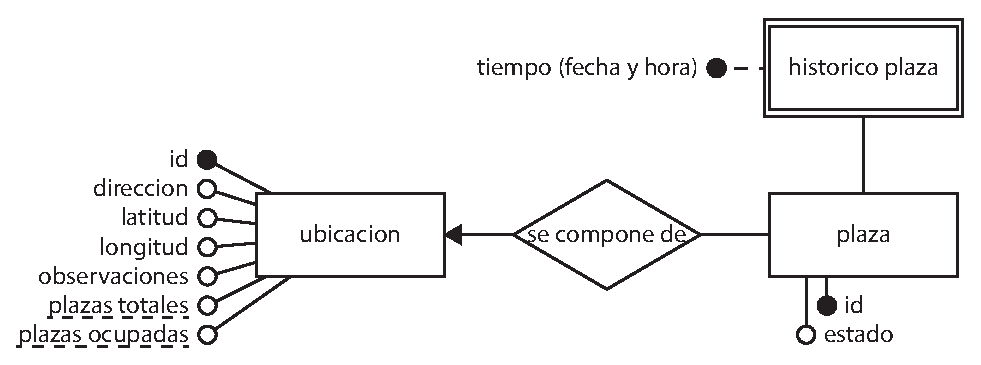
\includegraphics[width=0.7\textwidth]{imagenes/er_objetivo_4.eps}
	\caption{Esquema entidad-relación del objetivo 4}
	\label{er_objetivo_4}
\end{figure}
Por eficiencia del sistema y para saber cuántas de las plazas de una ubicación están ocupadas, se ha añadido un nuevo campo a las ubicaciones. Dicho campo se actualizará automáticamente según varíe el estado de las plazas de la ubicación.
\\\\
Una vez creadas las distintas tablas, en la API REST hay que crear los modelos para hacer un buen uso de estas tablas. Estos modelos tienen que tratar los datos en base a los casos de uso relacionados con el objetivo. Es por ello que, de momento, se tiene que dar de alta (añadir) plazas o ubicaciones, dar de baja (eliminar) plazas o ubicaciones y permitir modificar una ubicación existente. Además, se tendrá que visualizar la información contenida en el sistema, por lo que se debería sacar un listado de plazas y ubicaciones.
\\\\
Dicha funcionalidades en la API REST se tienen que materializar para que se pueda crear en la aplicación de gestión la parte de administración de plazas. Estas funcionalidades se han materializado de la siguiente forma:
\begin{itemize}
	\item Para dar de alta plazas se ha abierto la URI \textit{/plaza/nueva} con el método POST que recibe un JSON con el campo \textit{id\_ubicación}.
	\item Para dar de alta ubicaciones se ha abierto la URI \textit{/ubicacion/nueva} con el método POST que recibe un JSON con los campos \textit{direccion}, \textit{latitud}, \textit{longitud} y \textit{observaciones}.
	\item Para dar de baja una plaza se ha abierto la URI \textit{/plaza/<id>} con el método DELETE donde \textit{<id>} es el identificador de la plaza a eliminar.
	\item Para dar de baja una ubicación se ha abierto la URI \textit{/ubicacion/<id>} con el método DELETE donde \textit{<id>} es el identificador de la ubicación a eliminar.
	\item Para modificar una ubicación se ha abierto la URI \textit{/ubicacion/<id>} con el método POST donde \textit{<id>} es el identificador de la ubicación a modificar y recibe un JSON con los campos \textit{direccion} y \textit{observaciones}.
\end{itemize}
Todas estas funcionalidades devuelven un objeto JSON con un campo \textit{estado} que toma un valor booleano indicando si se ha podido realizar la operación. Al dar de alta una plaza, su estado es ``no definido'' y se actualiza el número de plazas totales de la ubicación donde se crea la plaza. De igual manera, cuando se elimina, se disminuye el número de plazas totales de la ubicación.
\\\\
De forma parecida, cuando se da de alta una ubicación, tanto el número de plazas totales como el de plazas ocupadas es cero. Y para eliminar una, estos dos campos deben estar a cero, es decir, que se hayan eliminado las plazas pertenecientes a la ubicación a eliminar.
\\\\
Para listar plazas y ubicaciones, las URIs son:
\begin{itemize}
	\item \textit{/plazas}, con método GET, que devuelve un objeto JSON con los campos \textit{num\_plazas} y \textit{plazas} que es una lista de objetos con los campos \textit{id}, \textit{estado} e \textit{id\_ubicacion}. 
	\item \textit{/ubicaciones} que devuelve un objeto JSON con los campos \textit{num\_ubicaciones} y \textit{ubicaciones}, con método GET, que es una lista de objetos con los campos \textit{id}, \textit{direccion}, \textit{latitud}, \textit{longitud}, \textit{plazas\_totales}, \textit{plazas\_ocupadas} y \textit{observaciones}. 
\end{itemize}
A las ubicaciones se le ha añadido un campo más en la tabla para saber qué número de sus plazas se encuentran ocupadas, \textit{plazas\_ocupadas}. Esta información va a ser útil de cara al usuario final de la aplicación móvil.
\\\\
Una vez que se encuentran hechas las funcionalidades en la API REST, en la aplicación de gestión hay que crear dos secciones: una que se encargue de la administración de las plazas y otra haga lo propio sobre las ubicaciones. Por supuesto, ambas páginas se actualizaran periódicamente para mostrar al administrador la ocupación real de las plazas que también se puede ver reflejada en las ubicaciones.
\\\\
También, los formularios para añadir plazas o ubicaciones, así como para modificar una ubicación, han sido validados tanto en el lado del cliente como en el lado de la API REST.
\\\\
Por otro lado, para facilitar la administración de las ubicaciones, se ha optado por incluir un mapa tanto en el listado de las ubicaciones como en la creación y modificación de la ubicación. Este mapa ha sido posible incluirlo a través de la API de Google \textit{Maps JavaScipt API} \cite{google-maps-js-api}.

\section{OBJ-5}
De igual manera que se ha hecho en el OBJ-4 se va a proceder en la implementación de éste. Lo primero es mirar en la matriz de trazabilidad, figura \ref{trazOBJ-R}, con qué requisitos de información y casos de uso está relacionado. Podemos ver que el OBJ-5 está relacionado con el requisito de información IRQ-3 y los casos de uso UC-7 y UC-8.
\\\\
Al igual que se ha hecho anteriormente, se debe hacer un esquema entidad-relación con la información que brinda el IRQ-3. Este esquema es el que se puede ver en la figura \ref{er_objetivo_5}.
\begin{figure}[H]
	\centering
	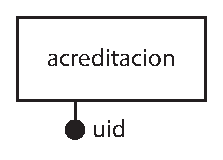
\includegraphics[width=0.15\textwidth]{imagenes/er_objetivo_5.eps}
	\caption{Esquema entidad-relación del objetivo 5}
	\label{er_objetivo_5}
\end{figure}
Como se puede observar, por ahora, sólo se guarda el identificador de la acreditación en el sistema. Esto hace que el sistema en sí no contenga datos de carácter personal ni información disgregada, ya que con esta información se podría llegar a saber la identidad de una persona.
\\\\
Este identificador (UID) es el identificador de la tarjeta pasiva RFID según el estándar ISO/IEC 15693 \cite{rfid-uid}. Dicho campo es de sólo lectura y único. También se puede ver el formato y la longitud de este identificador, que va a servir para verificar que el vehículo que ocupe una plaza monitorizada tiene autorización para ello.
\\\\
Una vez creada la tabla en la base de datos, así como su modelo y controlador en la API REST, las URIs que ésta tiene públicas para la administración de acreditaciones son:
\begin{itemize}
	\item \textit{/acreditaciones}, con método GET, que devuelve JSON con los campos \textit{num\_acreditaciones} y \textit{acreditaciones} que es un listado de las mismas. Dichas acreditaciones sólo tienen un campo que es \textit{uid}.
	\item \textit{/acreditacion/nueva}, con método POST, que recibe un JSON con el campo \textit{uid} y devuelve si se ha creado correctamente la nueva acreditación en el sistema.
	\item \textit{/acreditacion/<uid>}, con método DELETE, donde \textit{<uid>} es el UID de la tarjeta RFID que se quiere eliminar del sistema.
\end{itemize}
Una vez que se han publicado las URIs en la API REST, hacer la página de gestión de acreditaciones en la aplicación web de gestión no es tarea especialmente compleja. Además, y para evitar sobrecargas innecesarias, esta información no necesita actualizarse de forma periódica puesto que, para cambiar dicha información, el administrador necesita realizar acciones en dicha página.

\section{OBJ-6}
Esta parte del proyecto es vital debido a que el sistema tiene que tener información verídica del estado de ocupación de las plazas de aparcamiento. Para ello se va a proceder a crear un prototipo de agente de captación con sensores que actualice en tiempo real la información del sistema.
\\\\
Para ello, la primera decisión que hay que tomar es qué microcontrolador elegir. Tal y como se ha expuesto en el análisis, sección \ref{requisito-hw}, este microcontrolador debería disponer de WiFi para poder conectarse de manera inmediata con la API REST.
\\\\
El microcontrolador con WiFi que actualmente está revolucionando el mundo IoT (Internet of things, Internet de las cosas) a nivel doméstico, al estar presente en la electrónica de casi todos los dispositivos ``inteligentes'', es el ESP8266 \cite{esp8266}. Éste se puede encontrar en multitud de placas de desarrollo, entre ellas NodeMCU \cite{nodemcu}, Adafruit Huzzah \cite{huzzah}, SparkFun \cite{sparkfun-esp8266} o Wemos. Tanto Adafruit como SparkFun son dos de las grandes empresas de componentes de electrónica a nivel mundial que también tienen implicación por enseñar la llamada cultura \textit{maker}.
\\\\
Principalmente por motivo presupuestario pero sin obviar su funcionalidad, para este prototipo se ha optado por elegir la placa \textit{D1 mini Pro} de Wemos \cite{d1}. Esta placa presenta WiFi integrado, 11 pines de los cuales uno de ellos es analógico y dos de ellos son de trasmisión de datos y tres pines de alimentación (tierra, 5V y 3.3V).
\\\\
Una vez que ya está elegida la placa de desarrollo, el paso siguiente es ver cómo se puede programar. Este microcontrolador tiene la capacidad de poderse programar en NodeMCU \cite{nodemcu-firmware} (proveniente de Lua \cite{lua}), MicroPython \cite{micropython} o Arduino \cite{arduino}. Dado que NodeMCU y MicroPython son ambos lenguajes interpretados, se ha optado por programar al microcontrolador en Arduino.
\\\\
En NodeMCU y MicroPython lo que se hace es re-programar la memoria del microcontrolador con un intérprete que va leyendo el programa de la memoria y actúa en consecuencia. Esto hace que la velocidad de ejecución disminuya además de los problemas de seguridad relacionados al tener el código fuente en la memoria de la placa.
\\\\
Ahora que se sabe qué placa de desarrollo utilizar y cómo programarla, es el momento de buscar los sensores necesarios para la creación del prototipo. Para ello se va a elegir un receptor RFID para leer la credencial del usuario, si dispone, y un sensor de ultrasonidos para detectar al vehículo. 
\\\\
Con respecto al receptor RFID, se va a empezar por un dispositivo pequeño que sirva de ilustración en este prototipo. El receptor que más se utiliza es el MFRC522 \cite{rfid-especs}. Existen numerosas placas ya montadas para la creación de prototipos con este receptor. Una de ellas, y la más común, es RFID-RC522 \cite{rfid-modulo}.
\\\\
Dicho módulo se comunica con el microcontrolador a través de un BUS SPI que es un BUS síncrono, full dúplex con cuatro líneas \cite{spi}. Dichas lineas son:
\begin{itemize}
	\item SCK: línea de reloj.
	\item MOSI: línea de trasmisión maestro-esclavo.
	\item MISO: línea de trasmisión esclavo-maestro.
	\item SS: línea de selección del esclavo.
\end{itemize}
Realmente el microcontrolador ESP8266 soporta tan solo un dispositivo conectado a este BUS de acorde con su documentación \cite{esp8266-pins}.
\\\\
Siguiendo con la elección de los dispositivos hardware y antes de entrar a programar el agente de captación de datos, falta por seleccionar el sensor de ultrasonidos. Se puede ver en una búsqueda rápida que el más usado para la creación de prototipos es el HC-SR04 \cite{hcsr04}.
\\\\
El funcionamiento por el cual este sensor calcula la distancia entre él y un objeto es midiendo el tiempo de rebote de una onda sonora. Como se sabe que la velocidad del sonido en condiciones óptimas en la atmósfera terrestre es de $343m/s$, se puede calcular la distancia despejando la ecuación del movimiento rectilíneo uniforme: $$Distancia = Tiempo \times Velocidad$$ Dicha distancia sería la recorrida por el sonido desde que sale del sensor, rebota en el objeto y llega al sensor, por lo que la distancia entre el sensor y el objeto sería la mitad.
\\\\
Una vez que están los componentes del agente de captación de datos, el siguiente paso es proceder al montaje de dichos componentes:
\begin{itemize}
	\item RFID-RC522:
	\begin{itemize}
		\item 3.3V - Wemos 3.3V
		\item RST  - Wemos D3
		\item GND  - Wemos GND
		\item IRQ
		\item MISO - Wemos D6
		\item MOSI - Wemos D7
		\item SCK  - Wemos D5
		\item SDA  - Wemos D8
	\end{itemize}
	\item HC-SR04:
	\begin{itemize}
		\item VCC  - Wemos 5V
		\item Trig - Wemos D1
		\item Echo - Wemos D2
		\item GND  - Wemos GND
	\end{itemize}
	\item LED verde: Wemos RX - GND
	\item LED rojo: Wemos TX - GND
\end{itemize}
\begin{figure}[H]
	\centering
	\includegraphics[width=\textwidth]{imagenes/esquema_agente_captacion.pdf}
	\caption{Vista montaje agente de captación de datos}
	\label{esquema-agente-captacion}
\end{figure}
Como se puede ver, se han añadido dos LEDs, uno rojo y otro verde, que sirven para saber cuál es el estado de la plaza. Si el verde queda fijo, la plaza se encuentra bien ocupada. En cambio, si el rojo se queda fijo, la plaza está mal ocupada. Cuando ambos están apagados significa que la plaza está libre y si se encuentran parpadeando alternativamente es que se ha producido algún tipo de fallo en la comunicación con el servidor.
\\\\
Antes de entrar a programar el microcontrolador es necesario añadir dos URIs en la API REST:
\begin{itemize}
	\item \textit{/plaza/<id>/estado/<nuevo\_estado>}, con método PUT, donde \textit{<id>} es el identificador de la plaza de aparcamiento que se quiere cambiar el estado y \textit{<nuevo\_estado>} es el estado al que ha cambiado la plaza. Se devuelve un JSON con el identificador de la plaza y un booleano que indica si se ha actualizado correctamente.
	\item \textit{/acreditacion/<uid>}, con método GET, donde \textit{<uid>} es el UID de una tarjeta que se quiere comprobar que existe en el sistema. Se devuelve un JSON con el campo \textit{estado} a \textit{True} si existe y un error 404 en caso contrario.
\end{itemize}
La funcionalidad de la segunda es trivial. Sin embargo, la de la primera, no tanto. Ésta tiene que comprobar que el identificador de la plaza exista en el sistema y el nuevo estado sea distinto al del anterior para evitar posibles paquetes perdidos. Una vez que pase dichas comprobaciones tendrá, por una parte que actualizar, si procede, las plazas ocupadas de la ubicación donde se encuentra la plaza. Por otra parte tendrá que añadir en el histórico que se ha producido un cambio de estado en la plaza. Y, finalmente, actualizar el estado de la plaza en su tabla.
\\\\
\newpage
Una vez que se han añadido las dos URIs con su funcionalidad correspondiente a la API REST, se puede proceder a la programación del microcontrolador con Arduino, un lenguaje parecido a C, al cual se le puede añadir funcionalidades haciendo librerías en C/C++.
\\\\
Por suerte, Arduino ya tiene implementadas bastantes librerías. Una de ellas es SPI para poder usar el lector RFID. Además de las propias, hay contribuciones externas como es el caso de la librería ESP8266, para usar este microcontrolador en Arduino; MFRC522, para usar el lector RFID; o ArduinoJson para trabajar con objetos JSON.
\\\\
Aunque haya muchas funcionalidades hechas, programar un microcontrolador, no es tarea fácil debido a que, sólo tiene una hebra de ejecución. Por este motivo, se tiene que hacer de manera óptima para que parezca que es capaz de ejecutar varias tareas a la vez. Estas tareas van a ser: leer la distancia del sensor de ultrasonidos, leer el UID de la tarjeta cuando el sensor de ultrasonidos detecte un vehículo y el aparcamiento no esté actualizado, comprobar enviando una petición al servidor si la acreditación leída existe y actualizar el estado enviando otra petición al servidor en consecuencia con lo anterior.
\\\\
Como no va a estar constantemente midiendo la distancia, se ha programado una interrupción de reloj, cada cinco segundos, para proceder a esta acción. El único proceso donde el microcontrolador tiene que realizar una espera activa, y por tanto se nota que no funciona en tiempo real, es cuando se conecta con el servidor para hacer peticiones.
\\\\
En el lector RFID se podría colocar una línea de interrupción (pin IRQ) para que avise al microcontrolador en el momento de leer una tarjeta. Esta interrupción se ha optado por no hacerla debido a que, para leer la tarjeta, se tiene que hacer una petición expresa para ver si está detectándola.
\\\\
Por último, hay que establecer una distancia de detección, esto es, el módulo HC-SR04 va a medir la distancia hasta el primer objeto que se encuentre en un rango de 2cm a 4 metros. Si el objeto se encuentra más alejado de la distancia de detección, la plaza de aparcamiento estaría libre. En cambio, si éste se encuentra más cerca de la distancia de detección se infiere que hay un vehículo ocupando la plaza. También, se podría establecer un valor mínimo y así comprobar que el objeto se encuentra en un rango, por ejemplo la altura de los bajos de un vehículo.
\\\\
Con todo esto y una vez hecho el programa, se procede a programar el microcontrolador y a comprobar que funcione correctamente tanto la detección, a través de los sensores, como la conexión a la API REST. Con esto, el siguiente paso es modificar la aplicación de gestión para recibir alertas.

\section{OBJ-3}
Una vez que el agente de captación está creado y se han programado las distintas funcionalidades en la API REST, se va a proceder a crear un script, en la aplicación de gestión, para recibir alertas cuando alguna plaza esté mal ocupada. Pero antes de eso, hay que crear la funcionalidad en el servidor.
\\\\
Como en la tabla \textit{histórico plaza} se va guardando el estado de una plaza junto con la marca de tiempo cuando cambia, hay que ver aquí qué plazas están mal ocupadas para así sacar desde cuándo están mal ocupadas. La consulta para ello sería compuesta sacando el último estado de las plazas en esta tabla. Para ello se tiene que usar la cláusula \textit{distinct} en el identificador de la plaza. Después de esta primera consulta, la siguiente sería seleccionar aquellas tuplas cuyo estado sea \textit{mal ocupada}.
\\\\
Una vez que se ha creado la funcionalidad en el servidor y abierta la URI,\\
\textit{/plazas/mal\_ocupadas}, con método GET, que devuelve un JSON con el listado de plazas junto a la marca de tiempo de ocupación y cuyo estado es \textit{mal ocupada}, se puede proceder a sacar alertas en la aplicación.
\\\\
Para este último paso, se ha decidido usar una librería de muestra de notificaciones usando Bootstrap, Bootstrap Notify \cite{bootstrap-notify} bajo licencia MIT. Éstas mostrarán un mensaje en la parte superior derecha de la pantalla con aquellos identificadores de plazas junto a la hora y fecha del momento en el cual han sido mal ocupadas. Al pinchar en dicha notificación, la aplicación mostrará la página de administración de plazas.
\\\\
Estas notificaciones, al igual que la información de las plazas, se actualiza cada 10 segundos que es un intervalo de tiempo razonadamente corto y evita sobrecargar el servidor.

\section{OBJ-7}
Una vez que el sistema está funcionando y se puede administrar, el último paso de este proyecto es la creación de una aplicación móvil para el usuario final. Antes y hacer el caso de uso procedente, UC-10, hay que elegir con qué tecnología se va a crear dicha aplicación.
\\\\
A día de hoy existen diversos frameworks de desarrollo que permiten hacer una aplicación móvil multiplataforma, esto es, un único desarrollo daría como resultado varias aplicaciones: una para Android, otra para IOS y otra para Windows Phone. También se pueden hacer aplicaciones llamada Web-APPS con Ionic \cite{ionic} o con PhoneGap \cite{phonegap} entre otros muchos frameworks de desarrollo de ese estilo que hacen una aplicación a través de usar tecnología web.
\\\\
En ambos casos lo que realmente se está haciendo es \textit{transpilar}, es decir, generar un lenguaje a partir de otro para así hacer una aplicación. Aunque el desarrollo, en muchos casos, es más rápido y multiplataforma, la aplicación definitiva es más ineficiente que una desarrollada a mano. Por otro lado, tras actualizaciones en las plataformas de desarrollo (Android o IOS) hay muchos problemas al hacer una aplicación que necesite algún componente específico que es el caso de la aplicación que aquí se va a hacer. 
\\\\
Esto se dice porque, en primera instancia para desarrollar la aplicación móvil, se optó por Xamarin. Éste es un framework para desarrollar aplicaciones móvil multiplataforma propiedad de Microsoft. El desarrollo fue fácil al tener experiencia en C\# pero en el momento de necesitar componentes específicos como un mapa para poder las ubicaciones de aparcamiento en la aplicación, el desarrollo quedó estancado debido a que el gestor de paquetes de Xamarin no podía resolver las dependencias de algunos de ellos tras la actualización de la API de Google Maps. Dicha incidencia supuso un atraso en el desarrollo.
\\\\
Tras la mala experiencia, se decidió cambiar de mentalidad y desarrollar la aplicación de forma nativa para una sola plataforma: Android.
\\\\
Nada más comenzar a crear el proyecto en Android Studio para hacer la aplicación, después de elegir la plataforma base para el proyecto, hay que elegir un \textit{Activity} base. En dichos \textit{Activities}, por defecto hay una donde muestra un mapa de Google Maps.
\\\\
Lo primero que se tendría que hacer es mostrar en dicho mapa las ubicaciones de aparcamiento. Este listado de ubicaciones puede ser el mismo que se hizo para la aplicación pero, de esta manera sería ineficiente y presentaría un gasto de transmisión muy grande actualizar la información de la aplicación.
\\\\
Para resolver este problema y al sólo necesitar los datos de aquellas ubicaciones localizadas dentro de una zona determinada, ventana de visualización del mapa, se puede hacer diferentes peticiones dependiendo de la zona que se muestre en la aplicación. Por este motivo es necesario añadir una nueva URI con esta funcionalidad a la API REST.
\\\\
Esta nueva URI es:
\\
\textit{/ubicaciones/<lat\_min>\&<lat\_max>/<long\_min>\&<long\_max>}, con método GET, donde \textit{lat\_min} y \textit{long\_min} es la latitud y longitud de la esquina superior derecha y \textit{lat\_max} y \textit{long\_max} es lo propio de la esquina inferior izquierda de la zona visible de un mapa. Este método devuelve una un JSON con el número de ubicaciones incluidas en esa zona y un listado de ellas.
\\\\
Con esta nueva funcionalidad en la API REST, la aplicación móvil puede hacer una petición al servidor al detectar que se ha movido, ampliado o alejado el mapa, es decir, cuando ha habido algún tipo de cambio en la visualización del mismo. Para la conexión con el servidor se ha optado por usar, la librería de Android, Volley \cite{volley}.
\\\\
Una vez que se tiene los datos en la aplicación móvil, se tienen que visualizar. Para ello se tiene que usar la API de desarrollo de Google \cite{android-maps}. Antes de continuar, para poder hacer todo esto y poder visualizar correctamente el mapa en la aplicación, se debe obtener una \textit{API key} y activarla en la cuenta de desarrollador de Google.
\\\\
Ahora que se puede visualizar correctamente el mapa con las ubicaciones de aparcamiento, se procede a la creación de dos nuevos \textit{Activities}. El primero se va a mostrar cuando el usuario seleccione una ubicación del mapa. En este caso se le mostrará una pantalla con los datos actualizados de dicha ubicación y un botón para navegar hasta ella. El segundo se activará cuando el usuario marque otra posición distinta en el mapa. Este caso es el OBJ-8.
\\\\
Antes de proceder con él, hay que saber cómo navegar hasta la ubicación deseada. Para ello, lo que se ha pensado es hacer uso de la navegación de la aplicación Google Maps, que viene instalada en Android por defecto. Para ello se deben usar los \textit{intents} de Google Maps \cite{android-maps-intent}.
\\\\
Por último, se debería informar al usuario cuando se encuentra navegando a una ubicación si dicha ubicación se queda sin plazas disponibles. Para esto, la única solución es usando un servicio de notificaciones.
\\\\
Google también lo tiene solucionado con su servicio \textit{Cloud Messaging} ahora en Firebase \cite{firebase}. Este servicio se integra perfectamente con Android y, por parte del servidor, tiene SDK para python -\textit{firebase-admin}-.
\\\\
Pero para mandar la notificación se necesita saber a quién y cuándo mandarla. En respuesta a cuándo se mandaría sería en el momento que se actualice el estado de una plaza, en el caso de que la plaza quedase ocupada y fuese la última en esa ubicación. Para dar respuesta al quién, se necesita guardar en el servidor el destino del usuario junto al token que se usa en Firebase para mandar notificaciones a usuarios. Dicho token es único por dispositivo, es decir, un identificador.
\\\\
Es por ello que esta meta de desarrollo está relacionada con el requisito de información IRQ-6. Esta nueva información encajaría de la siguiente manera en la base de datos:
\begin{figure}[H]
	\centering
	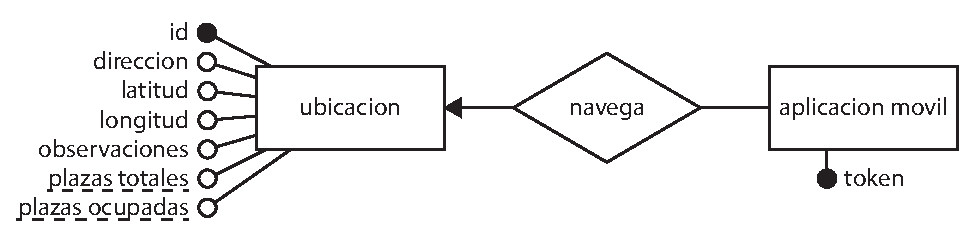
\includegraphics[width=0.7\textwidth]{imagenes/er_objetivo_7.eps}
	\caption{Esquema entidad-relación del objetivo 7}
	\label{er_objetivo_7}
\end{figure}
Una vez creada la tabla, hay que hacer su modelo y controlador en la API REST. Dicho controlador tendría las siguientes URIs abiertas:
\begin{itemize}
	\item \textit{/destino\_activo/nueva}, con método POST, que recibe un JSON con los campos \textit{id\_ubicacion} que es el identificador de ubicación donde el usuario se dispone a ir y \textit{token} que es el identificador del dispositivo del usuario. Esta funcionalidad da de alta un destino activo en el sistema.
	\item \textit{/destino\_activo/<token>}, con método DELETE, donde \textit{<token>} es el identificador del dispositivo del usuario para eliminarlo del sistema de notificaciones.
\end{itemize}
Estas dos funcionalidades devuelven un objeto JSON para afirmar si la operación se ha realizado correctamente. A la primera URI la aplicación móvil la llamaría justo antes de crear el intent de Google Maps para navegar. A la segunda, se llamaría al volver de Google Maps a la aplicación o al volver a abrir la aplicación.

\section{OBJ-8}
Para que la aplicación sea más útil, se ha pensado en que muestre una lista de ubicaciones cuando el usuario selecciona un destino en el municipio. A partir de ese destino, el sistema deberá escoger las mejores ubicaciones de aparcamiento para el usuario.
\\\\
Antes de explicar cómo se filtran las ubicaciones que se muestran en la lista, se puede observar en la matriz de trazabilidad, figura \ref{trazOBJ-R}, que este objetivo está relacionado con el requisito de información IRQ-5. Esto se debe a que se quiere recoger datos para un posterior estudio de la localización de las plazas en base al destino real de los usuarios que las usan. Estos datos se recogen de forma anónima en la siguiente tabla, sacada a partir de las especificaciones del requisito de información IRQ-5:
\begin{figure}[H]
	\centering
	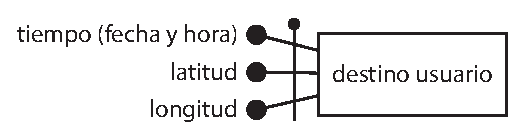
\includegraphics[width=0.4\textwidth]{imagenes/er_objetivo_8.eps}
	\caption{Esquema entidad-relación del objetivo 8}
	\label{er_objetivo_8}
\end{figure}
Esta tabla se va rellenando con los diferentes destinos de los usuarios cuando éstos hacen búsquedas en la aplicación. Pero para que se pueda hacer esto, es necesario crear la funcionalidad en la API REST que reciba las coordenadas de destino del usuario y le devuelva una lista de ubicaciones donde poder aparcar. Esta URI sería: \textit{/destinos\_usuario/nueva<lat>\&<long>}, con método PUT, siendo \textit{<lat>} y \textit{<long>} la latitud y longitud, respectivamente, del destino del usuario.
\\\\
\newpage
Por otro lado, la pantalla de la aplicación móvil que muestra un listado de ubicaciones dado el destino del usuario también necesita de una funcionalidad en la API REST para obtener dicho listado. Estas URI serían:
\begin{itemize}
	\item \textit{/ubicaciones/<lat>\&<long>}, con método GET, siendo \textit{<lat>} y \textit{<long>} la latitud y longitud, respectivamente, del destino del usuario.
	\item \textit{/ubicaciones/<lat>\&<long>/<grano>}, con método GET, siendo \textit{<lat>} y \textit{<long>} la latitud y longitud, respectivamente, del destino del usuario y \textit{<grano>} una distancia en metros para agrupar ubicaciones.
\end{itemize}
Ambas URIs devuelven una lista ordenada de ubicaciones.
\\\\
En la primera, el parámetro \textit{grano} se define a 0. Este parámetro ayuda a reordenar las ubicaciones. En principio, cuando el parámetro es 0, las ubicaciones se ordenan por distancia al destino marcado por el usuario. El parámetro lo que hace es crear grupos de ubicación que estén en el mismo rango de distancia con respecto al destino. Dentro de estos grupo las ubicaciones se ordenan por número de plazas disponibles. 
\\\\
Esto da lugar a que, si el valor del parámetro incrementa, aquellas ubicaciones que se encuentren más lejos del destino pero que tengan un mayor número de plazas libres, van a ir apareciendo en primeras posiciones. Es elección del usuario darle valor a dicho parámetro teniendo en cuenta cuánto se quiere desplazar.
\\\\
Para afinar el filtrado de las ubicaciones se ha pensado en utilizar un histórico de ocupación de las ubicaciones en base al histórico de ocupación de las plazas. Con esta información se podría elaborar un porcentaje de ocupación de una determinada zona en el tiempo.
\\\\
Por tanto, como las personas en general tenemos patrones de comportamiento, con el porcentaje anteriormente detallado se puede hacer una predicción del estado de ocupación de una ubicación en el futuro. Esto serviría para decirle al usuario cómo estará la ubicación cuando vaya a aparcar o serviría para que el sistema dirija al usuario a la ubicación donde tiene más probabilidades para estacionar, en base al tiempo que tardaría en llegar al lugar.
\\\\
Pero no todo hay que basarlo en el histórico, sino que, a su vez, datos como la climatología o los eventos de una ciudad, pueden estar relacionados con la ocupación de estos aparcamientos. Es por esto que el sistema va a quedar preparado para adaptar esta información para afinar la lista de ubicaciones que se le brinda al cliente.
\\\\
Puesto que para hacer esto se necesitarían bastantes datos, se pensó en la creación de un generador de datos que se comporte de manera esperada a como lo harían los usuarios de este tipo de aparcamientos. Este generador sería lo suficientemente complejo para suponer otro TFG, por lo que queda para un trabajo futuro junto con la integración de un agente con una base de conocimiento mayor que prediga la ocupación de la ubicación en el futuro.